% !TeX program = lualatex
\documentclass[UTF8,fontset=fandol,11pt,a4paper]{ctexart}
\usepackage[margin=24mm,headheight=15pt]{geometry}
\usepackage{fontspec}
\setmainfont{texgyretermes-regular.otf}[BoldFont=texgyretermes-bold.otf,ItalicFont=texgyretermes-italic.otf,BoldItalicFont=texgyretermes-bolditalic.otf]
\setsansfont{texgyreheros-regular.otf}[BoldFont=texgyreheros-bold.otf]
\setmonofont{lmmono10-regular.otf}[Scale=MatchLowercase]
\usepackage{amsmath,amssymb,bm,mathtools,graphicx,booktabs,tabularx,longtable,array}
\usepackage{float,placeins,xurl}
\usepackage[numbers,sort&compress]{natbib}
\usepackage{xcolor,hyperref,fancyhdr}
\definecolor{inkblue}{HTML}{245781}
\hypersetup{colorlinks=true,linkcolor=inkblue,citecolor=inkblue,urlcolor=inkblue,
  pdftitle={Deep CORAL 的扩展探索：多层对齐、权重自适应与 LMMD 对照实验},pdfauthor={张以禾}}
\pagestyle{fancy}
\fancyhf{}
\fancyhead[L]{\small Deep CORAL 的扩展探索}
\fancyhead[R]{\small Office-31：Amazon $\to$ Webcam}
\fancyfoot[C]{\thepage}
\renewcommand{\headrulewidth}{0.3pt}
\setlength{\parindent}{2em}
\setlength{\parskip}{0.25em}
\linespread{1.12}
\raggedbottom
\setlength{\emergencystretch}{2em}
\setlength{\textfloatsep}{13pt plus 3pt minus 3pt}
\setlength{\floatsep}{11pt plus 3pt minus 3pt}
\renewcommand{\arraystretch}{1.15}
\graphicspath{{figures/}}
\newcolumntype{Y}{>{\raggedright\arraybackslash}X}
\newcommand{\CE}{\mathcal L_{\mathrm{CE}}}
\newcommand{\sg}{\operatorname{sg}}
\newcommand{\norm}[1]{\left\lVert #1\right\rVert}
\newcommand{\ESS}{\operatorname{ESS}}
\newcommand{\file}[1]{\texttt{\nolinkurl{#1}}}
\newcommand{\pp}{\,\text{pp}}
\newcommand{\LayersRows}{%
conv5+fc8 & 55.09 & +0.88 & 55.35 / 28 \\
fc7+fc8 & 54.34 & +0.13 & 54.34 / 45 \\
fc8 & 54.21 & +0.00 & 54.21 / 37 \\
fc6+fc8 & 52.33 & -1.89 & 52.96 / 33 \\
fc6+fc7+fc8 & 51.82 & -2.39 & 52.08 / 33 \\
conv5 & 50.82 & -3.40 & 50.82 / 33 \\
No adaptation & 46.54 & -7.67 & 48.05 / 3 \\
fc7 & 45.91 & -8.30 & 46.92 / 45 \\
fc6+fc7 & 45.41 & -8.81 & 45.66 / 14 \\
fc6 & 44.40 & -9.81 & 46.67 / 22 \\
}

\newcommand{\WeightsRows}{%
fc8：固定 & 50 & 54.21 / 37 & 54.21 & 0.500 \\
conv5+fc8：固定 & 100 & 56.48 / 58 & 52.58 & 0.500 \\
fc8：第 1 轮起自适应 & 50 & 54.97 / 28 & 51.32 & 3.645 \\
fc8：第 41 轮起自适应 & 50 & 54.21 / 37 & 53.58 & 0.866 \\
conv5+fc8：第 50 轮起自适应 & 100 & 55.97 / 58 & 53.58 & 6.936 \\
}

\newcommand{\SubdomainRows}{%
no\_adaptation & $0$ & 46.54 & 46.60 \\
global & $0.5G$ & 53.84 & 53.39 \\
global\_quarter & $0.25G$ & 54.09 & 53.67 \\
local & $0.5L_C$ & 42.14 & 43.22 \\
mixed & $0.25G+0.25L_C$ & 49.56 & 49.85 \\
lmmd & $0.5M$ & 66.16 & 66.16 \\
}

\newcommand{\ResnetRows}{%
no\_coral & 100 & 80.00 & 80.00 & +0.00 \\
logits & 37 & 81.01 & 78.49 & +2.52 \\
pooled & 100 & 80.38 & 80.00 & +0.38 \\
pooled\_logits & 42 & 80.25 & 78.11 & +2.14 \\
layer4 & 100 & 79.87 & 80.00 & -0.13 \\
layer4\_logits & 42 & 81.76 & 78.11 & +3.65 \\
}

\newcommand{\GeometryRows}{%
global & 0.12058 & 0.326 & 10.11 & 0.427 \\
local & 0.01053 & 0.331 & 5.14 & 0.229 \\
lmmd & 0.03481 & 0.102 & 7.82 & 0.591 \\
}

\newcommand{\InventoryRows}{%
1 & AlexNet CORAL & no\_adaptation\_fixed\_50 & 50 & 300 \\
2 & AlexNet CORAL & fc8\_fixed\_50 & 50 & 300 \\
3 & AlexNet CORAL & fc6\_fixed\_50 & 50 & 300 \\
4 & AlexNet CORAL & fc6\_fc7\_fixed\_50 & 50 & 300 \\
5 & AlexNet CORAL & fc6\_fc7\_fc8\_fixed\_50 & 50 & 300 \\
6 & AlexNet CORAL & fc6\_fc8\_fixed\_50 & 50 & 300 \\
7 & AlexNet CORAL & fc7\_fixed\_50 & 50 & 300 \\
8 & AlexNet CORAL & fc7\_fc8\_fixed\_50 & 50 & 300 \\
9 & AlexNet CORAL & conv5\_fixed\_50 & 50 & 300 \\
10 & AlexNet CORAL & conv5\_fc8\_fixed\_50 & 50 & 300 \\
11 & AlexNet CORAL & joint\_fixed\_100 & 100 & 600 \\
12 & AlexNet CORAL & fc8\_adaptive\_full\_50 & 50 & 300 \\
13 & AlexNet CORAL & fc8\_adaptive\_delayed\_50 & 50 & 300 \\
14 & AlexNet CORAL & joint\_adaptive\_delayed\_100 & 100 & 600 \\
15 & ResNet50 CORAL & no\_coral & 100 & 2400 \\
16 & ResNet50 CORAL & logits & 37 & 888 \\
17 & ResNet50 CORAL & pooled & 100 & 2400 \\
18 & ResNet50 CORAL & pooled\_logits & 42 & 1008 \\
19 & ResNet50 CORAL & layer4 & 100 & 2400 \\
20 & ResNet50 CORAL & layer4\_logits & 42 & 1008 \\
21 & AlexNet subdomain & no\_adaptation & 50 & 300 \\
22 & AlexNet subdomain & global & 50 & 300 \\
23 & AlexNet subdomain & global\_quarter & 50 & 300 \\
24 & AlexNet subdomain & local & 50 & 300 \\
25 & AlexNet subdomain & mixed & 50 & 300 \\
26 & AlexNet subdomain & lmmd & 50 & 300 \\
27 & ResNet50 LMMD & author\_code\_seed42 & 72 & 6264 \\
}

\title{\bfseries Deep CORAL 的扩展探索\\[3pt]\large 多层对齐、权重自适应与 LMMD 对照实验}
\author{张以禾}
\date{2026 年 10 月 30 日}
\begin{document}
\maketitle
\begin{abstract}
无监督域适应通过利用目标域的无标签图像，改善源域模型在分布变化后的分类表现。本研究围绕 Deep CORAL 的扩展开展四个阶段的探索：增加对齐层、学习适应权重、替换预训练网络，以及比较类别条件下的协方差匹配与核分布匹配。在 Office-31 Amazon$\to$Webcam 的归档实验中，多层 CORAL 的最佳固定轮配置为 conv5+fc8，准确率 55.09\%，相对 fc8 增加 0.88 个百分点，但增加层数没有形成一致收益；基于梯度范数的自适应权重未形成稳定改善，并伴随权重增长和梯度方向冲突。ResNet-50 V2 在共享 BatchNorm 下的无 CORAL 对照达到 80.00\%，含 logits 的 CORAL 配置取得 2.14--3.65 个百分点的同轮增益。进一步的 AlexNet 匹配对照中，类条件 CORAL 与 LMMD 分别达到 42.14\% 和 66.16\%，全局 CORAL 为 53.84\%；独立的 ResNet LMMD 配方获得 93.71\% 的目标标签选轮结果。实验与事后诊断表明，对齐层数、权重大小和协方差距离都不能单独代表迁移质量；统计目标是否保留类别位置、软分组是否可靠，以及比较协议是否一致，是解释结果的关键。本文逐阶段记录实验结论与反思，并据此总结可检验的改进方向。
\end{abstract}
\noindent\textbf{关键词：}无监督域适应；Deep CORAL；多层对齐；自适应权重；LMMD；实验分析
\section*{引言与实验约定}

深度模型在源域上获得较高分类准确率，并不意味着其特征能够直接迁移到成像条件不同的目标域。Deep CORAL 将源域分类损失与跨域协方差距离联合优化，为这一问题提供了结构简洁的训练目标\cite{sun2016deep}。这一设计也留下了直接的探索空间：把约束加到更多层、根据训练状态自动调整强度，或者使用更强的特征网络，是否会进一步改善迁移？当这些扩展没有形成预期收益时，问题又出在优化强度、特征表示，还是对齐的统计对象？

本文沿这条问题链组织四部分实验。第一部分比较不同层及层组合，检验增加约束位置的收益；第二部分尝试梯度范数平衡，并用固定权重日志分析训练何时应当结束；第三部分更换为 ResNet-50，观察强预训练与共享 BatchNorm 条件下 CORAL 的额外作用；第四部分转向类别条件对齐，比较自定义类条件 CORAL 与 DSAN 的 LMMD\cite{zhu2021dsan}，通过结果与数学性质反思统计目标的选择。各部分按照“探索与实验—阶段结论与反思”展开，后续探索由前一部分留下的问题引出。

全部实验使用 Office-31 的 Amazon$\to$Webcam 方向，31 类；源域包含 2,817 张图像，目标域包含 795 张图像，随机种子均为 42。目标准确率对全部 795 张图像计算，差值以百分点（pp）表示。源域准确率来自训练图片上的全量评估。本文整理截至 2026 年 10 月 12 日的 27 个归档运行，共 1,593 轮、22,968 次参数更新；本次论文整理没有新增训练。原汇报中的“Deep CORAL 原实验复现”在此指本地实现的基线实验，不表示与原论文全部训练设置逐项相同。

各阶段采用各自的结果选择方式：AlexNet 位置实验与子域对照以固定第 50 轮为主；100 轮权重实验同时呈现最终值与历史最佳值；ResNet CORAL 报告损失规则决定的停止轮，并与无 CORAL 对照的相同轮次比较；ResNet LMMD 按目标域准确率选择最佳模型。表中历史最佳值与固定轮结果分别列示。

\textbf{目标标签的用途随实验协议披露。}所有适应损失均不读取目标真实标签。AlexNet 的历史探索已查看目标评估曲线，损失早停规则的部分设计也参考了既有曲线；子域六组在阶段内固定协议与第 50 轮结果，目标真值用于评估及事后诊断；ResNet LMMD 则明确用目标真值进行最佳轮选择及 30 轮无提升停止。因此，后者的 93.71\% 属于目标标签参与模型选择的结果。所有结果均为单种子、单迁移方向的观察，本文据此比较具体配置和提出机制解释，不估计跨种子显著性。

\section{多层 CORAL：增加对齐位置能否改善迁移？}
\label{sec:multi}

\subsection{探索动机与实验设计}

Deep CORAL 在分类输出上施加二阶统计约束，并给出了多层损失的联合形式\cite{sun2016deep}。不同深度的表示包含不同信息：卷积层反映局部通道响应，较深的全连接层逐渐形成类别表征。因此，本阶段从 fc8 单层基线出发，探索卷积统计与输出统计是否互补，以及同时对齐多个全连接层能否减少残留域差异。

对于某层的特征矩阵 $Z_d\in\mathbb R^{n_d\times D}$，$d\in\{s,t\}$，记 $H_n=I_n-\mathbf1^\top/n$，则协方差与 CORAL 损失为
\begin{equation*}
 C_d=\frac{Z_d^\top H_{n_d}Z_d}{n_d-1},\qquad
 G_\ell=\frac{\norm{C_s^{(\ell)}-C_t^{(\ell)}}_F^2}{4D_\ell^2}.
\end{equation*}
选定层集合 $\mathcal A$ 后，本实验对各层损失取均值：
\begin{equation*}
 \mathcal L=\CE+\lambda G,\qquad
 G=\frac{1}{|\mathcal A|}\sum_{\ell\in\mathcal A}G_\ell,
 \qquad\lambda=0.5.
 \label{eq:multi}
\end{equation*}
因此，单层系数为 0.5，双层各为 0.25，三层各为 $1/6$。这一约定固定总系数，却没有固定每个已有层的系数。

模型为 ImageNet V1 预训练 AlexNet，fc8 改为 31 类输出。fc6、fc7 使用 ReLU 前的 4,096 维 Linear 输出，fc8 使用 31 维 logits；conv5 使用 ReLU 前的 256 维通道响应，将批次内空间位置合并为 $BHW$ 个观测后计算通道协方差。空间观测存在相关性，观测数量增加不等同于增加独立图像样本。

十组配置使用 batch=128、固定 50 轮，每轮由较短域配对产生 6 次更新。SGD 主干及 fc6/fc7 学习率为 0.001，fc8 为 0.01，momentum=0.9，weight decay=$5\times10^{-4}$；采用原始图像、Resize(224) 和按域归一化，不增加随机裁剪或翻转。训练为确定性 FP32，关闭 TF32，Windows 数据加载 workers=0。

\subsection{实验结果}

基线曲线见图\ref{fig:baseline}。第 50 轮，无适应组为 46.54\%，fc8 CORAL 为 54.21\%，相差 7.67 pp。源域分类能够较快拟合，但源域拟合程度和目标域表现没有同步变化；引入 fc8 CORAL 后，输出层协方差距离得到控制，并伴随更高的目标准确率。这一观察支持以 fc8 作为后续位置探索的参照。

\begin{figure}[H]
 \centering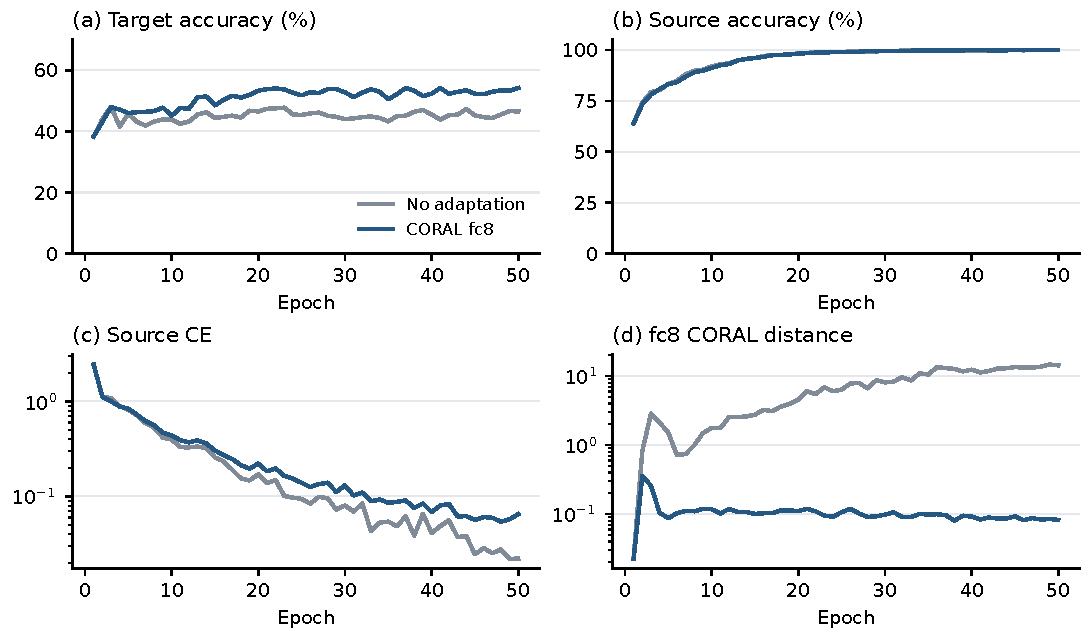
\includegraphics[width=\linewidth]{baseline.pdf}
 \caption{AlexNet 基线实验。两组均训练至第 50 轮；(c)(d) 为对数纵轴。无适应组的 CORAL 距离作为监测量记录，不参与该组反向传播。}
 \label{fig:baseline}
\end{figure}

\begin{table}[H]
 \centering\small
 \caption{多层 CORAL 的完整位置比较。准确率单位为 \%；差值为相对 fc8 第 50 轮的百分点差。最佳值来自历史目标评估，作为补充。}
 \label{tab:layers}
 \begin{tabular}{lrrr}
 \toprule
 对齐位置 & 第 50 轮 & 相对 fc8（pp） & 最佳值 / 轮次\\
 \midrule
 \LayersRows
 \bottomrule
 \end{tabular}
\end{table}

表\ref{tab:layers}与图\ref{fig:layers}给出了所有组合。conv5+fc8 达到 55.09\%，相对 fc8 为 $+0.88\pp$；fc7+fc8 为 54.34\%，相对 fc8 为 $+0.13\pp$。其余全连接联合设置没有形成同样的增益：fc6+fc8 为 52.33\%，fc6+fc7+fc8 为 51.82\%，fc6+fc7 为 45.41\%。单独 fc6、fc7 的结果为 44.40\%、45.91\%。增加层数并未带来单调改善。

\begin{figure}[H]
 \centering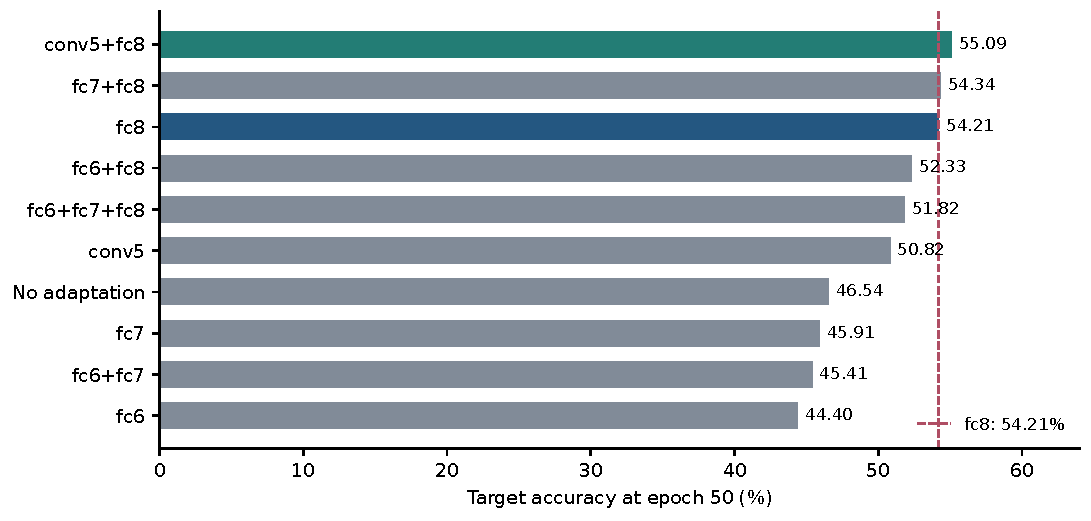
\includegraphics[width=.94\linewidth]{layers.pdf}
 \caption{固定第 50 轮的位置实验。虚线表示 fc8 参照；所有柱均从零起绘制。conv5+fc8 的局部增益与多数多层组合缺少收益这两个事实同时成立。}
 \label{fig:layers}
\end{figure}

\subsection{阶段结论与反思}

\textbf{本阶段没有得到“更多层联合对齐可以有效改善迁移”的结论。}conv5+fc8 提供了 0.88 pp 的正向观察，但这一收益尚没有多种子证据；把它扩展为多层方法的一般优势，会超出当前实验。相反，十组结果说明，对齐位置的选择比层数本身更值得关注。

失败分析首先涉及\textbf{统计估计与任务语义的关系}。batch=128 时，4,096 维图像特征的样本协方差秩至多为 127；全连接层还受到训练态 Dropout 的影响。高维、低秩、带随机扰动的统计量未必稳定刻画需要消除的域变化。fc8 对齐直接作用于类别输出，conv5 则使用另一种局部通道统计，两者可能形成互补。这些是与结构和结果一致的解释，实验没有单独改变 batch、Dropout 或估计器，尚不能识别其中哪项构成主要原因。

另一个关键是\textbf{层位置与层权重发生了联动}。式\eqref{eq:multi}在增加一层时，同时降低已有层的系数；例如 fc8 从单层的 0.5 变为双层的 0.25。因此，联合组与单层组比较的是完整配置，并非“保持 fc8 不变后再加一项”的纯消融。若后续检验层间互补，应固定已有层系数，再单独扫描新增层；还应记录逐层梯度的范数和方向，而非根据不同维度下的原始 CORAL 数值排名。

这一阶段保留的工作参照是固定权重的 fc8 与 conv5+fc8。随后的问题转向：如果固定的总系数没有在训练全过程维持合适的优化关系，能否由训练信号自动学习它？

\FloatBarrier
\section{自适应 \texorpdfstring{$\lambda$}{λ}：梯度范数平衡为何没有形成稳定收益？}
\label{sec:adaptive}

\subsection{探索动机与权重学习方法}

分类与对齐损失的梯度会随训练改变，固定 $\lambda$ 未必使两项约束始终保持相近影响。本阶段借鉴 GradNorm 的梯度平衡思路\cite{chen2018gradnorm}，在共享 conv5 参数上监测两项损失的梯度范数，并学习正的适应权重。这里仅实现范数匹配控制器。

记共享参数上的梯度为 $g_{\mathrm{CE}}=\nabla_\theta\CE$、$g_G=\nabla_\theta G$，对其范数维护 decay=0.9 的指数滑动平均（EMA），以 $s=\log\lambda$ 参数化正权重，最小化
\begin{equation*}
 J_\lambda=\left(e^s\overline{\norm{g_G}_2}-\overline{\norm{g_{\mathrm{CE}}}_2}\right)^2.
 \label{eq:controller}
\end{equation*}
独立 Adam 以学习率 0.01 更新 $s$，权重裁剪在 $[10^{-4},100]$ 内；模型更新使用停止梯度的 $\lambda$。初值为 0.5，预热阶段固定权重、更新范数统计。实验覆盖 fc8 全程自适应、最后 20\% 轮次自适应，以及 conv5+fc8 第 50 轮起自适应；与相同预算的固定权重组比较。

\subsection{实验结果与训练轨迹}

表\ref{tab:lambda}同时给出最佳值与最终值。fc8 全程自适应的峰值为 54.97\%，第 50 轮为 51.32\%；固定组为 54.21\%。第 41 轮才开始学习的 fc8 最终为 53.58\%，其最佳值出现在第 37 轮，即权重学习开始之前。延迟启动没有改变这一配置的最佳记录。

\begin{table}[H]
 \centering\small
 \caption{固定与自适应权重实验。准确率单位为 \%；末次 $\lambda$ 是最后一步权重更新后的值，不同于最后一轮使用权重的均值。}
 \label{tab:lambda}
 \begin{tabular}{lrrrr}
 \toprule
 配置 & 轮数 & 最佳值 / 轮次 & 最终值 & 末次 $\lambda$\\
 \midrule
 \WeightsRows
 \bottomrule
 \end{tabular}
\end{table}

对于 conv5+fc8 的 100 轮对照，固定组第 58 轮达到 56.48\%，最终为 52.58\%；延后自适应组第 58 轮达到 55.97\%，最终为 53.58\%。自适应组的末轮多 1.01 pp，峰值则少 0.50 pp。因此，这组数据既不能被概括为所有指标都变差，也不能支持稳定改善：两种结果选择方式给出了不同方向的差值。

\begin{figure}[H]
 \centering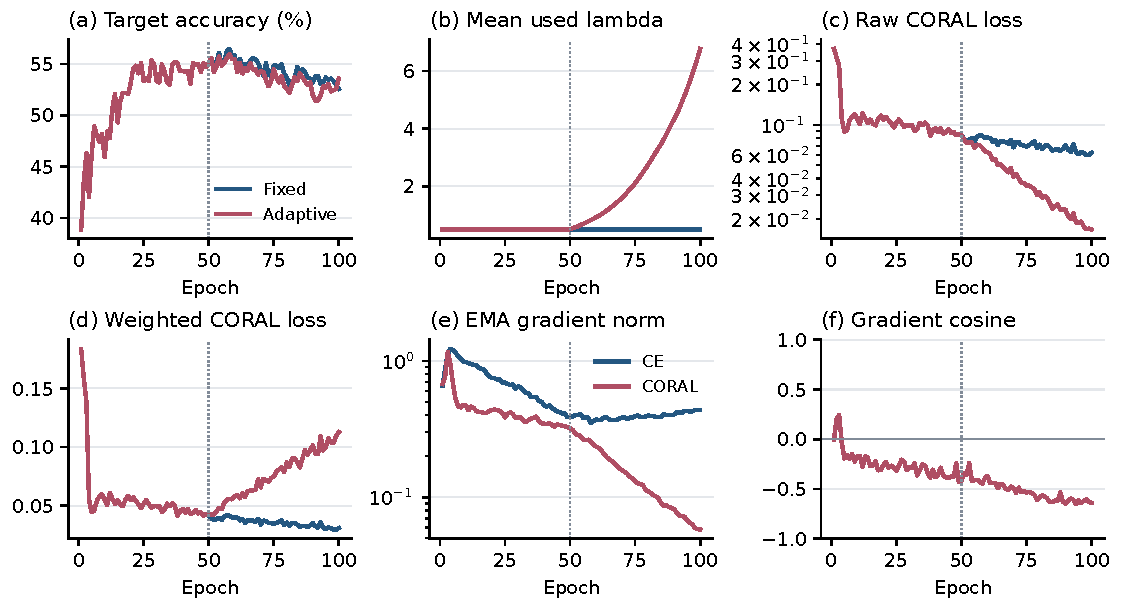
\includegraphics[width=\linewidth]{adaptive.pdf}
 \caption{conv5+fc8 固定与延后自适应的 100 轮轨迹。虚线为第 50 轮启用位置。梯度统计取自共享 conv5 参数，(e) 是范数 EMA，(f) 为逐批梯度余弦的轮均值。曲线未平滑或补点；图 (b) 为实际使用权重的轮均值。}
 \label{fig:adaptive}
\end{figure}

两组前 49 轮的分类损失、CORAL 损失与准确率在 $10^{-6}$ 容差内一致。图\ref{fig:adaptive}显示，开启自适应后，控制器不断增加权重：末次更新后 $\lambda$ 为 6.94，第 100 轮实际使用权重的均值为 6.77。原始 $G$ 从第 49 轮约 0.0853、第 50 轮 0.0837，变为第 100 轮 0.0167；与此同时，加权项没有按同样比例变小，第 100 轮 $\lambda G$ 的逐批均值为 0.11267，分类损失为 0.09619。

\subsection{失败分析：平衡了大小，没有处理方向}

\textbf{权重上升符合控制器自身的目标。}第 50 轮的平均 EMA 范数比 $\overline{\norm{g_{\mathrm{CE}}}}/\overline{\norm{g_G}}$ 约为 1.21，第 100 轮约为 7.53。随着 CORAL 梯度变小，式\eqref{eq:controller}要求更大的 $\lambda$ 才能补足范数差距。权重没有达到上界，现有记录也没有非有限优化失败；更直接的问题是控制器的目标与目标域分类质量并不等价。

\textbf{两项梯度存在方向冲突。}自适应组第 100 轮的梯度余弦均值为 $-0.641$，第 50 轮为 $-0.415$。对忽略动量与权重衰减的一次理想化梯度步，有
\begin{equation*}
 \Delta\CE\approx-\eta\left(\norm{g_{\mathrm{CE}}}_2^2
       +\lambda\langle g_{\mathrm{CE}},g_G\rangle\right).
 \label{eq:direction}
\end{equation*}
当内积为负时，提高对齐权重会抵消一部分源域分类下降方向；即使两项范数匹配，方向关系也不会因此改善。式\eqref{eq:direction}说明该控制目标遗漏了什么，但它不是目标误差变化的因果估计。实际更新还包含动量、权重衰减和其余网络参数，轮均范数与轮均余弦也不能直接代入还原每步内积。

此外，原始 CORAL 变小既可能来自有效匹配，也可能来自表示尺度变化。当前自适应实验没有保存足够的特征几何诊断，不能把图\ref{fig:adaptive}中的损失下降直接称为特征坍塌。Deep CORAL 原文关于单独优化对齐项可能出现退化解的讨论\cite{sun2016deep}提供了需要检查的方向，而不是对本次训练状态的证明。

\subsection{阶段结论与反思}

本阶段不保留这套自适应控制器作为有效改进方案。它提高了原始对齐目标的优化压力，却没有带来稳定的分类收益；\textbf{把范数匹配当作优化目标，需要同时检查梯度方向与表示几何}。只在共享 conv5 上测量的统计也不能代表所有层的更新关系。

\FloatBarrier
\section{更换网络：强预训练下 CORAL 还提供什么？}
\label{sec:backbone}

\subsection{探索动机与实验设计}

前两部分表明，继续增加约束或调节强度并没有形成一致收益。由此转向表示本身：使用更强的预训练主干之后，目标域表现是否改善，CORAL 是否仍能提供可辨认的额外作用？本阶段将 AlexNet 换为 ImageNet V2 预训练 ResNet-50，比较无 CORAL、logits、pooled、layer4 及两种含 logits 的联合设置。

logits 为 31 维输出；pooled 为 2,048 维全局空间均值；layer4 为末级残差相加及 ReLU 后的空间通道特征。layer4 仍将空间位置合并后估计通道协方差。固定 $\lambda=0.5$，多层取均值；SGD 主干学习率 0.001、分类头 0.01，momentum 与 weight decay 沿用前述设置。batch 调整为 32，每轮 24 次更新，输入使用 Resize(224) 和按域归一化。五个 CORAL 组使用第二部分的训练损失停止规则，未触发则运行 100 轮；无 CORAL 组运行至 100 轮。

\textbf{无 CORAL 对照采用相同的共享 BatchNorm。}每步按源域、目标域顺序前向，两域均更新 BN 统计量；评估时冻结。即使不使用适应损失，目标域输入也已影响模型。

\subsection{实验结果与停止信号}

表\ref{tab:resnet}与图\ref{fig:resnet}报告停止轮表现。无 CORAL 组第 100 轮为 80.00\%。pooled 与 layer4 单独对齐均跑满 100 轮，准确率为 80.38\% 与 79.87\%，同轮差值为 $+0.38\pp$ 与 $-0.13\pp$。这两种特征统计约束在当前协议下没有提供清晰的额外分类收益。

\begin{table}[H]
 \centering\small
 \caption{ResNet-50 V2 的 CORAL 比较。准确率单位为 \%。同轮对照取无 CORAL 组在对应停止轮的准确率，不统一减去其第 100 轮结果。}
 \label{tab:resnet}
 \begin{tabular}{lrrrr}
 \toprule
 配置 & 停止轮 & 准确率 & 同轮对照 & 差值（pp）\\
 \midrule
 \ResnetRows
 \bottomrule
 \end{tabular}
\end{table}

含 logits 的三个配置观察到正向同轮收益：logits 第 37 轮为 81.01\%，对照为 78.49\%；pooled+logits 第 42 轮为 80.25\%，对照为 78.11\%；layer4+logits 第 42 轮为 81.76\%，对照为 78.11\%。相应增益为 2.52、2.14、3.65 pp。这说明强预训练下 CORAL 的作用依赖对齐位置，且 CORAL 在这一预训练网络上的效果已经微乎其微。

\begin{figure}[H]
 \centering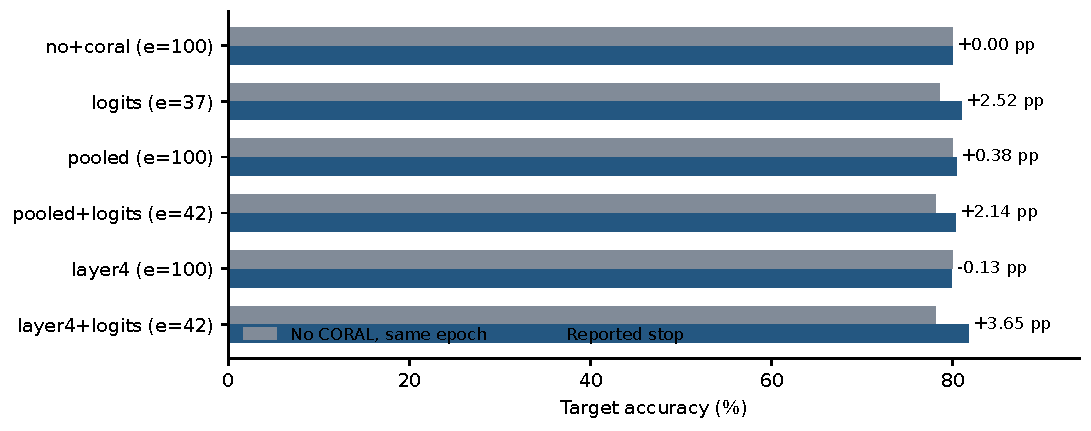
\includegraphics[width=\linewidth]{resnet_coral.pdf}
 \caption{ResNet CORAL 的停止轮及同轮对照。柱旁为同轮百分点差。无 CORAL 对照也利用目标图像更新 BN，全部横柱从零起绘制。}
 \label{fig:resnet}
\end{figure}

损失平衡与分类峰值也出现分离。三个含 logits 的组分别在第 37、42、42 轮停止，其目标准确率峰值却都出现在第 22 轮。相较之下，pooled 与 layer4 的最终加权 CORAL 项分别约为 CE 的 4.68\%、49.28\%，没有满足两项损失接近的停止条件。不同层的距离与梯度具有不同尺度，即使使用相同 $\lambda$，也不意味着相同的优化约束。

\subsection{阶段结论与反思}

更换网络后，无 CORAL 配置的目标准确率达到 80.00\%，实验表明预训练、微调和共享 BN 的组合能够形成较强的迁移参照。含 logits 的 CORAL 仍提供了可观察的同轮增益，而单独 pooled、layer4 没有形成同样的变化。考虑到此时 CORAL 带来的提升已经非常小了，我们转向另一个问题：全局二阶统计没有直接保留类别对应关系，能否通过选择更合适的对齐对象改善迁移？

\FloatBarrier
\section{寻找其他对齐方案比较：从类条件 CORAL 到 LMMD}
\label{sec:alternatives}

\subsection{探索一：把全局协方差匹配改为逐类匹配}

全局协方差同时包含类内变化和类间中心结构；不同类别的域偏移可能在整体统计中相互掩盖。DSAN 通过源域真实类别和目标预测概率建立相关子域，再以 LMMD 对齐其核分布\cite{zhu2021dsan}。本阶段先借用这种软类别分组思路，将统计目标换成逐类协方差，检验能否保留 CORAL 的简洁形式并获得更细的对齐。

在 AlexNet fc8 的 31 维 logits 上，源域权重由 one-hot 标签归一化，目标权重由预测概率归一化：
\begin{equation*}
 p_{jc}=\sg[\operatorname{softmax}(z_j^t)_c],\qquad
 a^s_{ic}=\frac{\mathbf1[y_i^s=c]}{\sum_r\mathbf1[y_r^s=c]},\qquad
 a^t_{jc}=\frac{p_{jc}}{\sum_rp_{rc}}.
\end{equation*}
目标概率停止梯度，但目标特征本身仍参与反向传播。对于被保留的类别，全部目标图像通过其软权重参与统计，top-1 类别用于支持筛选，不是硬分组后的样本截取。加权均值与协方差为
\begin{equation*}
 \mu_d^c=\sum_i a^d_{ic}z_i^d,\qquad
 C_d^c=\frac{\sum_i a^d_{ic}(z_i^d-\mu_d^c)(z_i^d-\mu_d^c)^\top}
 {1-\sum_i(a^d_{ic})^2}.
\end{equation*}
这一有限样本修正在均匀权重下还原样本协方差；特征依赖的软权重不保证总体无偏估计。有效类别集合 $\mathcal V$ 要求源样本数至少 2、目标 top-1 支持至少 2，且目标 $\ESS_c=1/\sum_j(a^t_{jc})^2\ge2$。自定义类条件损失为
\begin{equation*}
 L_C=\frac1{|\mathcal V|}\sum_{c\in\mathcal V}
 \frac{\norm{C_s^c-C_t^c}_F^2}{4D^2},\qquad D=31.
 \label{eq:local}
\end{equation*}
这不是 DSAN 原方法；DSAN 的原始统计目标是核均值嵌入。

\subsection{匹配对照与类条件 CORAL 的结果}

为隔离阶段内的训练差异，重新建立 AlexNet 六组对照，保持相同初始化、batch=128、每轮 6 步、SGD 与预处理，固定训练 50 轮。所有适应组前十轮均使用 $\CE+0.5G$，第 11 轮起切换到表\ref{tab:subdomain}中的适应项；无适应组保留目标前向，使 Dropout 的随机数消耗方式一致。各适应组的前十轮共同指标已在 $10^{-6}$ 容差内核对。

本阶段全局 CORAL 为 53.84\%，与第一部分历史 fc8 的 54.21\% 属于分别归档的运行族。阶段内比较使用重新建立的 53.84\% 对照，不能因表面配置相近而替换分母或拼接曲线。

\begin{table}[H]
 \centering\small
 \caption{AlexNet 子域六组匹配对照。准确率与宏平均类别准确率单位为 \%，均取固定第 50 轮。表中每组均含源域 CE；适应组第 1--10 轮为 $0.5G$。}
 \label{tab:subdomain}
 \begin{tabular}{lcrr}
 \toprule
 配置 & 第 11--50 轮适应项 & 准确率 & 宏平均\\
 \midrule
 \SubdomainRows
 \bottomrule
 \end{tabular}
\end{table}

把全局项完全替换为 $0.5L_C$ 后，准确率为 42.14\%，相对全局 CORAL 为 $-11.70\pp$。保留 $0.25G$ 并增加 $0.25L_C$ 的 mixed 为 49.56\%；相同全局系数、没有局部项的 global\_quarter 为 54.09\%，差值为 $-4.53\pp$。这一额外对照排除了“联合组只是因为全局权重减半”这一单独解释。逐图配对记录中，local 相对 global 修正 14 张，却新增 107 张错误，净差为 $-93$ 张；现象来自分类判定变化，而非结果表的四舍五入。

\subsection{探索二：保留软类别分组，改用 LMMD}

上述结果提出了更具体的问题：逐类划分本身是否不足，协方差目标是否遗漏了分类所需信息？为此追加一组 LMMD，复用五组已完成对照。该组同样经过十轮全局 CORAL 预热，第 11--50 轮改用 $\CE+0.5M$。模型、轮数、采样与初始化保持匹配，改变的是局部统计目标及其作者支持规则；它不是完整 DSAN 架构复现。

LMMD 使用相同的源域 one-hot 与目标软概率权重，在再生核 Hilbert 空间中匹配类别条件均值\cite{zhu2021dsan}：
\begin{equation}
\begin{aligned}
 M&=\frac1{|\mathcal U|}\sum_{c\in\mathcal U}
 \left\|\sum_i a^s_{ic}\phi(z_i^s)-\sum_j a^t_{jc}\phi(z_j^t)\right\|_{\mathcal H}^2,\\
 M_c&=\sum_{i,i'}a^s_{ic}a^s_{i'c}k(z_i^s,z_{i'}^s)
 +\sum_{j,j'}a^t_{jc}a^t_{j'c}k(z_j^t,z_{j'}^t)
 -2\sum_{i,j}a^s_{ic}a^t_{jc}k(z_i^s,z_j^t).
\end{aligned}
\label{eq:lmmd}
\end{equation}
作者代码以源真实类与目标 top-1 类的交集为 $\mathcal U$，每域出现一个支持样本即可，不设 ESS 门槛；域内求和保留对角线，使用 V-statistic。核为五个 RBF 核之和，带宽取拼接批次非对角平方距离的均值并停止梯度，具体公式见附录。该约定依照归档作者实现\cite{dsancode}，并非将论文的带宽文字描述直接当作代码行为。

\begin{figure}[H]
 \centering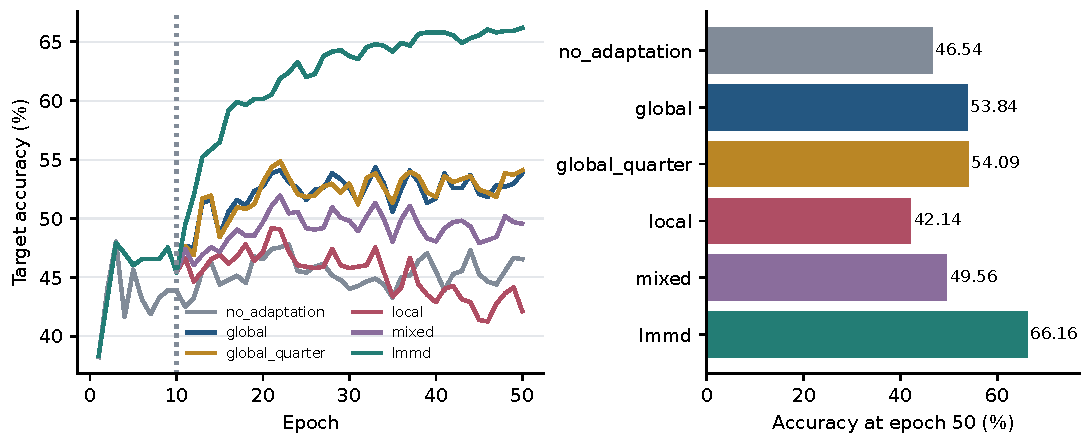
\includegraphics[width=\linewidth]{subdomain.pdf}
 \caption{AlexNet 六组训练与固定轮结果。虚线为十轮预热结束；LMMD 第 50 轮达到 66.16\%。全部适应组共享预热协议，阶段内全局对照为 53.84\%。}
 \label{fig:subdomain}
\end{figure}

LMMD 的第 50 轮准确率为 66.16\%，相对 global 为 $+12.33\pp$，相对 local 为 $+24.03\pp$。相对 global，LMMD 修正 119 张而新增 21 张错误，净增加 98 张正确预测；宏平均类别准确率同为 66.16\%。图\ref{fig:subdomain}表明，这一收益出现在预热后训练过程中。匹配对照支持继续研究“类别软分组与核分布匹配”的组合，而不是直接放弃类别条件对齐。

\subsection{结果反思：更小的协方差距离为何没有更好的分类？}

对六组固定最终模型进行全域 logits 诊断，关闭 Dropout，以真实类别计算协方差距离与中心方向；目标真值在此用于训练后的解释。表\ref{tab:geometry}及图\ref{fig:geometry}选择 global、local、LMMD 三组展示。

\begin{table}[H]
 \centering\small
 \caption{固定第 50 轮的事后几何诊断，使用原始 logits。$D_C$ 为真实类协方差距离，$D_{\rm dir}$ 为真实类中心余弦距离，$Q$ 为目标软类别权重纯度。距离对类别等权平均，定义见附录。}
 \label{tab:geometry}
 \begin{tabular}{lrrrr}
 \toprule
 配置 & $D_C$ & $D_{\rm dir}$ & 目标平均范数 & $Q$\\
 \midrule
 \GeometryRows
 \bottomrule
 \end{tabular}
\end{table}

\begin{figure}[H]
 \centering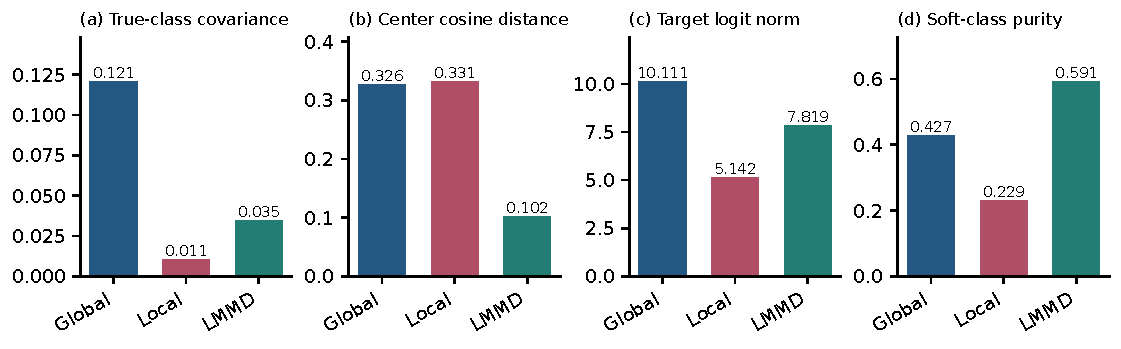
\includegraphics[width=\linewidth]{geometry.pdf}
 \caption{协方差、类别中心、幅度与软分组的联合诊断。local 的协方差距离最小；LMMD 的中心方向距离更小、软权重纯度更高。各面板独立标度，指标排序不等同于因果贡献。}
 \label{fig:geometry}
\end{figure}

\textbf{第一，类内协方差不直接约束类别中心。}固定类别权重时，各域独立平移不改变其协方差：
\begin{equation*}
 C_a(Z+\mathbf1v^\top)=C_a(Z).
\end{equation*}
即使源目标同类中心不同，类条件 CORAL 也可为零。local 的 $D_C$ 比 global 小约 91.3\%，中心方向距离却由 0.326 变为 0.331。LMMD 的 $D_C$ 为 0.03481，大于 local 的 0.01053，但中心方向距离为 0.102，分类准确率也更高。由此可见，减小类内波动差异与改善类别位置是不同目标。

\textbf{第二，绝对二阶距离具有尺度捷径。}固定权重、令两域表示共同缩放为 $sZ$，有 $L_C(sZ_s,sZ_t)=s^4L_C(Z_s,Z_t)$。local 的目标平均范数从 global 的 10.11 变为 5.14，目标协方差迹从 97.93 变为 24.27，与尺度收缩相符。不过，去除逐图共同 logit 偏移后的协方差形状距离也有所改善，说明二阶匹配变化不全由缩放解释；local 的目标有效秩为 25.19，且仍预测到全部 31 类，现有证据不支持将其称为低秩或单点坍塌。

进一步去除不影响 softmax 的共同 logit 偏移后，local 的类中心方向距离仍为 0.331，其归一化分类 margin 中位数为 $-0.086$，global 为 0.033；二者不会因共同正缩放而改变。目标类间协方差迹分别为 9.17 与 45.93，LMMD 为 39.45。较小的类内差异可以伴随类别间结构收缩，这比单看原始损失更贴近本次分类现象。

\textbf{第三，软权重的覆盖与纯度需要分开。}local 的软分组纯度为 0.229，global 为 0.427，LMMD 为 0.591；其全域平均 ESS 却从 global 的 60.30 增至 177.03。更大的 ESS 表示权重较分散，不表示集中于更多正确同类图像。被保留类别内，若概率对不同图像缺少区分，归一化软权重便接近均匀，其统计量会趋近全域统计而失去清晰类别含义。软分组混杂与局部约束可能形成相互强化的过程，这是与诊断一致、仍需干预实验检验的解释。

\textbf{第四，LMMD 改变了统计信息与类别利用方式。}线性核下式\eqref{eq:lmmd}就是类别中心差平方；RBF 核进一步感知非线性分布结构。固定带宽的高斯核在总体层面是特征核，MMD 为零可以识别分布相等\cite{gretton2012kernel}，但这一性质不等价于有限批次、预测软分组下的零分类误差。作者每批重估带宽时，在带宽下限未触发、类别权重固定的条件下，共同缩放不会改变核值；这一前向性质使 LMMD 的数值不因两域一起缩小而自动改善。带宽停止梯度意味着不能进一步把它解释为训练梯度的尺度不变性。

训练第 11--50 轮，local 按 CORAL 规则平均保留 21.92 类；LMMD 按作者规则为 29.37 类，同一 LMMD 运行按 CORAL 规则监测为 24.89 类。LMMD 不需要逐类协方差的双样本支持，因而可以利用更多共享类。同时，其加权损失量级也不同：第 50 轮为 0.41433，global 的加权 CORAL 为 0.04126。该比较没有匹配的适应梯度记录，不能把损失值之比当作梯度强度之比，也不能把收益全部归因于核函数。

\subsection{探索三：采用 ResNet-50 的 DSAN 作者代码配方}

AlexNet 的匹配实验给出了继续采用 LMMD 的依据。随后使用 ResNet-50 V2 与 256 维 bottleneck，按 DSAN 作者代码口径开展一组独立实验。模型为 $2048\to256\to31$，新增两层 Linear 之间不加 ReLU、Dropout 或 BN，对齐 256 维 bottleneck。该实验采用 batch=32、源域驱动的 87 步/轮、目标批次循环复用，不使用 CORAL 预热。

学习率按作者衰减，适应权重按预定训练进度渐增至 0.5；这与第二部分根据梯度反馈学习的自适应 $\lambda$ 是两种不同机制。训练输入采用 Resize(256)、随机裁剪至 224、随机水平翻转和 ToTensor，不增加 Normalize；评估为 Resize(224) 与 ToTensor。保留共享 BN，预算为 200 轮，每轮用目标准确率更新最佳记录，30 轮无严格提高即停止。

\begin{figure}[H]
 \centering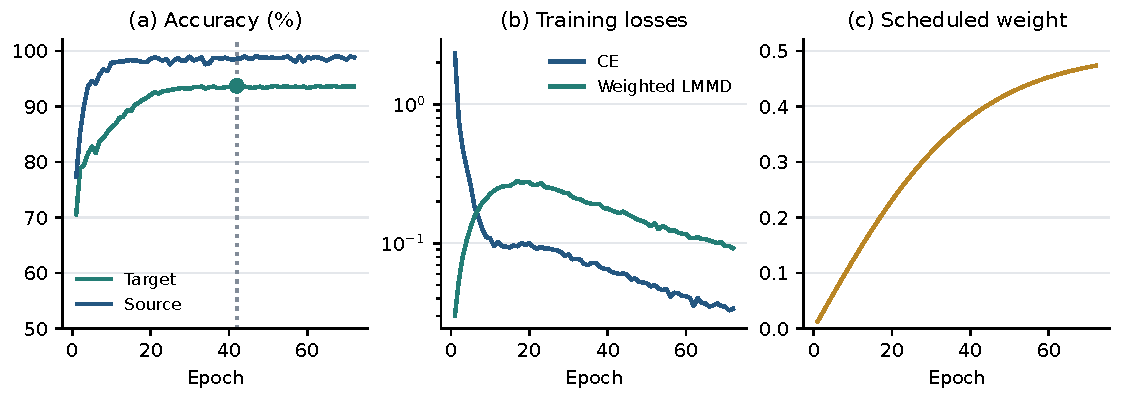
\includegraphics[width=\linewidth]{resnet_lmmd.pdf}
 \caption{ResNet-50 V2 的 LMMD 独立实验。第 42 轮最佳为 93.71\%，第 72 轮停止为 93.58\%；目标真值参与选轮和停止。右图为预设权重调度，不是梯度范数控制。}
 \label{fig:resnetlmmd}
\end{figure}

该组完成 72 轮、6,264 步，第 42 轮最佳为 93.71\%，第 72 轮停止为 93.58\%（图\ref{fig:resnetlmmd}）。DSAN 原论文报告 A$\to$W 为 $93.6\pm0.2\%$，对应三次随机实验的均值与标准误\cite{zhu2021dsan}；本地单次结果与其处于相近数值区间，但预训练、实现及选择条件不同，不能据此声称统计复现或超越。

与第三部分相比，本组同时改变了 bottleneck、增强、归一化、每轮步数、学习率、权重调度和结果选择方式。因而 93.71\% 与旧 CORAL 的 81.76\% 不构成匹配的损失替换对照，两者差值不能作为 LMMD 的独立收益。它说明的是这套完整配方的本地表现；LMMD 的阶段内直接比较依据仍是表\ref{tab:subdomain}。

\subsection{阶段结论与反思}

本阶段最清晰的结果是：\textbf{在匹配 AlexNet/fc8 与预热配置下，LMMD 达到 66.16\%，自定义类条件 CORAL 为 42.14\%。}类条件 CORAL 已改善真实类二阶统计，却没有改善分类；问题不能简单归为损失没有优化成功。中心位置、尺度以及软分组质量的诊断，将反思从“是否继续增加约束”推进到“统计目标是否约束了任务需要的信息”。

后续检验应围绕这些解释设置干预：统一两种局部损失的支持集合，以训练内梯度统计校准强度，再比较软类别均值匹配、协方差匹配及其联合；对软标签可靠性进行独立干预，观察纯度、中心方向与分类是否共同变化。LMMD 的优势也需要在这些因素固定后判断。由此保留 LMMD 作为继续探索的工作参照，并把类别几何与优化强度分开验证，而不是将任一事后诊断升级为普遍的性能代理。

\FloatBarrier
\section*{结语}

四部分探索逐步收紧了对有效对齐的判断标准。多层 CORAL 的结果表明，增加约束位置并不自动带来收益，层的语义及权重分配需要共同考虑；自适应 $\lambda$ 的结果表明，梯度范数相近不能解决方向冲突，也不能替代迁移质量判断；更换网络后的结果表明，强预训练与共享 BN 建立了较强参照，CORAL 的额外作用仍取决于对齐位置；类别条件对照则表明，减少二阶差异与改善分类可以分离，保留类别位置和可靠软分组的统计目标更值得继续检验。

\bibliographystyle{unsrtnat}
\bibliography{references}
\FloatBarrier
\appendix
\section{指标定义与训练配方}

\subsection{分类与几何指标}

目标准确率为 $N_t^{-1}\sum_j\mathbf1[\hat y_j=y_j]$，宏平均类别准确率先计算各类正确比例，再对 31 类等权平均。每一张目标图像对应约 $0.126\pp$。历史最佳值并列时取最早轮次。

令 $\widehat C_d^c,\widehat\mu_d^c$ 为冻结模型在全域真实类别 $c$ 上的普通样本协方差和均值，表\ref{tab:geometry}的指标为
\begin{align*}
 D_C&=\frac1{31}\sum_{c=1}^{31}\frac{\norm{\widehat C_s^c-\widehat C_t^c}_F^2}{4D^2},\\
 D_{\rm dir}&=\frac1{31}\sum_{c=1}^{31}
 \left(1-\frac{\langle\widehat\mu_s^c,\widehat\mu_t^c\rangle}
 {\norm{\widehat\mu_s^c}_2\norm{\widehat\mu_t^c}_2}\right),\\
 Q&=\frac1{31}\sum_{c=1}^{31}\sum_{j:y_j^t=c}
       \frac{p_{jc}}{\sum_rp_{rc}}.
\end{align*}
这些真实类诊断不同于训练时的软分组损失。$Q$ 表示每个预测软类别总权重中落在真实同类上的比例。余弦指标遇到零范数时按缺失记录；本表三组没有该类缺失。协方差形状距离以协方差矩阵的 Frobenius 内积定义对应余弦距离。

原始 logits 为 $z$，去共同偏移表示为 $\widetilde z=z-\mathbf1(\mathbf1^\top z)/D$，保持 softmax 概率与预测不变。归一化 margin 为
\begin{equation*}
 m(z,y)=\frac{z_y-\max_{c\ne y}z_c}{\norm{\widetilde z}_2}.
\end{equation*}
本文用其在目标域的中位数描述分类几何。协方差有效秩为 $\exp(-\sum_r q_r\log q_r)$，其中 $q_r$ 是非负特征值按和归一化后的谱权重；它描述谱的分散程度，不是语义类别数。

\subsection{LMMD 核与 ResNet 调度}

拼接一个源目标批次得到 $u_1,\ldots,u_n$，归档实现使用
\begin{equation*}
 b=\max\!\left(\sg\!\left[\frac{\sum_{r\ne q}\norm{u_r-u_q}_2^2}{n(n-1)}\right],10^{-12}\right),
 \qquad k(x,y)=\sum_{h=0}^{4}\exp\!\left(-\frac{\norm{x-y}_2^2}{b2^{h-2}}\right).
\end{equation*}
五核直接相加，不除以核数；无共享类时返回与特征梯度连接的零损失。作者损失的归档数值核验中，AlexNet 31 维对照损失误差为 0、最大特征梯度误差约 $2.24\times10^{-8}$；ResNet 256 维对照相应为 0 与 $5.82\times10^{-10}$。这些是既有实现核验，不是本次论文整理中新执行的训练。

ResNet LMMD 第 $e$ 轮的计划预算 $E=200$，学习率与适应权重为
\begin{equation*}
 \eta_g(e)=\frac{\eta_{g,0}}{(1+10(e-1)/200)^{0.75}},\qquad
 \lambda(e)=0.5\left(\frac{2}{1+\exp(-10e/200)}-1\right).
\end{equation*}
主干基础学习率为 0.001，bottleneck 与分类头为 0.01；SGD momentum=0.9，weight decay=$5\times10^{-4}$。作者循环保留 $\operatorname{range}(1,\operatorname{len}(\text{source loader}))$ 的行为，因此 88 个源完整批次对应 87 次更新。该轮定义不同于较短域配对的 24 步/轮。

\begin{table}[H]
 \centering\small
 \caption{跨阶段协议对照。第 4 列的选轮使用目标真实标签。所有 ResNet 组共享源、目标 BN；AlexNet 没有 BN。}
 \label{tab:protocol}
 \begin{tabularx}{\linewidth}{lYYY}
 \toprule
 项目 & AlexNet 子域六组 & ResNet CORAL & ResNet LMMD\\
 \midrule
 对齐表示 & 31 维 fc8 & pooled / layer4 / logits & 256 维 bottleneck\\
 batch / 每轮更新 & 128 / 6 & 32 / 24 & 32 / 87\\
 训练输入 & Resize 与按域归一化 & Resize 与按域归一化 & 裁剪、翻转，无 Normalize\\
 学习率 & 固定 & 固定 & 按轮衰减\\
 适应权重 & 十轮预热后固定 & 固定 0.5 & 预设渐增\\
 报告轮次 & 固定第 50 轮 & 训练损失停止轮 & 目标准确率最佳轮及停止轮\\
 \bottomrule
 \end{tabularx}
\end{table}

\section{归档运行清单与证据索引}

以下按运行而非展示表计数。第一部分的 fc8 同时出现在权重表中，不重复计数；子域实验另行训练的对照属于独立运行。清单共 27 组，其中 AlexNet CORAL/权重 14 组、ResNet CORAL 6 组、AlexNet 子域 6 组、ResNet LMMD 1 组。轮数记录实际完成长度；ResNet LMMD 的最佳轮为 42，而实际运行至 72。

\begingroup\scriptsize
\begin{longtable}{r p{29mm} p{69mm} rr}
\caption{全部归档运行及计算长度。}\label{tab:inventory}\\
\toprule
序号 & 实验族 & 运行标识 & 轮数 & 更新数\\
\midrule
\endfirsthead
\toprule 序号 & 实验族 & 运行标识 & 轮数 & 更新数\\\midrule
\endhead
\bottomrule\endfoot
\InventoryRows
\end{longtable}
\endgroup

本文基于 20 页汇报 \file{reports/PPT/2/main.pdf} 及其对应的 CSV、JSON、实验报告与实现整理。论文目录保留直接使用的 42 份输入快照，\file{data/sources.json} 记录仓库源路径与字节数；\file{reference/main.pdf} 保留汇报原件。正文图表由本地快照重绘，输入对应关系见 \file{data/figure_sources.json}。

\begin{table}[H]
 \centering\small
 \caption{论文目录内的主要证据。路径相对 \file{report/paper/}。}
 \begin{tabularx}{\linewidth}{lY}
 \toprule
 证据类别 & 文件与用途\\
 \midrule
 多层与权重 & \file{data/alex_layers.csv}、\file{data/alex_lambda.csv}、\file{data/alex_epochs.csv}、\file{data/alex_steps.csv}\\
 固定权重回放 & \file{data/early_stop.csv}、\file{data/early_stop_grid.csv}、\file{data/early_stop_epochs.csv}\\
 ResNet CORAL & \file{data/resnet_summary.csv}、\file{data/resnet_epochs.csv}\\
 子域分类对照 & \file{data/subdomain_summary.csv}、\file{data/subdomain_epochs.csv}、\file{data/subdomain_pairs.csv}\\
 子域诊断 & \file{data/subdomain_diagnostics.csv}、\file{data/subdomain_classes.csv}、\file{data/subdomain_phases.csv}\\
 ResNet LMMD & \file{data/resnet_lmmd_summary.json}、\file{data/resnet_lmmd_epochs.csv}\\
 公式与原协议 & \file{reference/} 中的损失实现、作者代码快照、历史协议及实验报告\\
 本次整理核验 & \file{data/validation.json}、\file{data/document_validation.json}\\
 \bottomrule
 \end{tabularx}
\end{table}

本次整理重新核对了结果表的正确数与准确率、AlexNet 最终与最佳轮记录、前 49 轮固定/自适应共同轨迹、首次损失平衡停止轮，以及 ResNet 同轮基线差值。历史模型推理与梯度公式核验的证据沿用归档 JSON，来源在清单中列明；没有重新训练、重载模型或重算全域 logits。\file{README.md} 说明材料结构和构建命令，\file{scripts/prepare.py} 从冻结证据重绘图表，不调用训练模块。

\end{document}
